% Options for packages loaded elsewhere
% Options for packages loaded elsewhere
\PassOptionsToPackage{unicode}{hyperref}
\PassOptionsToPackage{hyphens}{url}
\PassOptionsToPackage{dvipsnames,svgnames,x11names}{xcolor}
%
\documentclass[
  ignorenonframetext,
  aspectratio=169,
]{beamer}
\newif\ifbibliography
\usepackage{pgfpages}
\setbeamertemplate{caption}[numbered]
\setbeamertemplate{caption label separator}{: }
\setbeamercolor{caption name}{fg=normal text.fg}
\beamertemplatenavigationsymbolsempty
% remove section numbering
\setbeamertemplate{part page}{
  \centering
  \begin{beamercolorbox}[sep=16pt,center]{part title}
    \usebeamerfont{part title}\insertpart\par
  \end{beamercolorbox}
}
\setbeamertemplate{section page}{
  \centering
  \begin{beamercolorbox}[sep=12pt,center]{section title}
    \usebeamerfont{section title}\insertsection\par
  \end{beamercolorbox}
}
\setbeamertemplate{subsection page}{
  \centering
  \begin{beamercolorbox}[sep=8pt,center]{subsection title}
    \usebeamerfont{subsection title}\insertsubsection\par
  \end{beamercolorbox}
}
% Prevent slide breaks in the middle of a paragraph
\widowpenalties 1 10000
\raggedbottom
\AtBeginPart{
  \frame{\partpage}
}
\AtBeginSection{
  \ifbibliography
  \else
    \frame{\sectionpage}
  \fi
}
\AtBeginSubsection{
  \frame{\subsectionpage}
}
\usepackage{iftex}
\ifPDFTeX
  \usepackage[T1]{fontenc}
  \usepackage[utf8]{inputenc}
  \usepackage{textcomp} % provide euro and other symbols
\else % if luatex or xetex
  \usepackage{unicode-math} % this also loads fontspec
  \defaultfontfeatures{Scale=MatchLowercase}
  \defaultfontfeatures[\rmfamily]{Ligatures=TeX,Scale=1}
\fi
\usepackage{lmodern}

\useoutertheme[left]{sidebar}
\ifPDFTeX\else
  % xetex/luatex font selection
\fi
% Use upquote if available, for straight quotes in verbatim environments
\IfFileExists{upquote.sty}{\usepackage{upquote}}{}
\IfFileExists{microtype.sty}{% use microtype if available
  \usepackage[]{microtype}
  \UseMicrotypeSet[protrusion]{basicmath} % disable protrusion for tt fonts
}{}
\makeatletter
\@ifundefined{KOMAClassName}{% if non-KOMA class
  \IfFileExists{parskip.sty}{%
    \usepackage{parskip}
  }{% else
    \setlength{\parindent}{0pt}
    \setlength{\parskip}{6pt plus 2pt minus 1pt}}
}{% if KOMA class
  \KOMAoptions{parskip=half}}
\makeatother


\usepackage{longtable,booktabs,array}
\usepackage{calc} % for calculating minipage widths
\usepackage{caption}
% Make caption package work with longtable
\makeatletter
\def\fnum@table{\tablename~\thetable}
\makeatother
\usepackage{graphicx}
\makeatletter
\newsavebox\pandoc@box
\newcommand*\pandocbounded[1]{% scales image to fit in text height/width
  \sbox\pandoc@box{#1}%
  \Gscale@div\@tempa{\textheight}{\dimexpr\ht\pandoc@box+\dp\pandoc@box\relax}%
  \Gscale@div\@tempb{\linewidth}{\wd\pandoc@box}%
  \ifdim\@tempb\p@<\@tempa\p@\let\@tempa\@tempb\fi% select the smaller of both
  \ifdim\@tempa\p@<\p@\scalebox{\@tempa}{\usebox\pandoc@box}%
  \else\usebox{\pandoc@box}%
  \fi%
}
% Set default figure placement to htbp
\def\fps@figure{htbp}
\makeatother





\setlength{\emergencystretch}{3em} % prevent overfull lines

\providecommand{\tightlist}{%
  \setlength{\itemsep}{0pt}\setlength{\parskip}{0pt}}



 


\logo{
\includegraphics[width=1cm]{images/gw_logo.png}}
\setbeamertemplate{footline}[page number]
\usepackage{xcolor}
\definecolor{ApriBlue}{HTML}{0190DB}
\definecolor{Buff}{HTML}{AA9868}
\usepackage{theme/colortheme}
\usepackage[scaled]{helvet}
\usepackage[T1]{fontenc}
\makeatletter
\@ifpackageloaded{caption}{}{\usepackage{caption}}
\AtBeginDocument{%
\ifdefined\contentsname
  \renewcommand*\contentsname{Table of contents}
\else
  \newcommand\contentsname{Table of contents}
\fi
\ifdefined\listfigurename
  \renewcommand*\listfigurename{List of Figures}
\else
  \newcommand\listfigurename{List of Figures}
\fi
\ifdefined\listtablename
  \renewcommand*\listtablename{List of Tables}
\else
  \newcommand\listtablename{List of Tables}
\fi
\ifdefined\figurename
  \renewcommand*\figurename{Figure}
\else
  \newcommand\figurename{Figure}
\fi
\ifdefined\tablename
  \renewcommand*\tablename{Table}
\else
  \newcommand\tablename{Table}
\fi
}
\@ifpackageloaded{float}{}{\usepackage{float}}
\floatstyle{ruled}
\@ifundefined{c@chapter}{\newfloat{codelisting}{h}{lop}}{\newfloat{codelisting}{h}{lop}[chapter]}
\floatname{codelisting}{Listing}
\newcommand*\listoflistings{\listof{codelisting}{List of Listings}}
\makeatother
\makeatletter
\makeatother
\makeatletter
\@ifpackageloaded{caption}{}{\usepackage{caption}}
\@ifpackageloaded{subcaption}{}{\usepackage{subcaption}}
\makeatother

\usepackage{bookmark}
\IfFileExists{xurl.sty}{\usepackage{xurl}}{} % add URL line breaks if available
\urlstyle{same}
\hypersetup{
  pdftitle={Automated Prior Elicitation for Bayesian Metabolomics Analysis},
  pdfauthor={Chiraag Gohel},
  colorlinks=true,
  linkcolor={Buff},
  filecolor={Maroon},
  citecolor={Blue},
  urlcolor={ApriBlue},
  pdfcreator={LaTeX via pandoc}}


\title{Automated Prior Elicitation for Bayesian Metabolomics Analysis}
\subtitle{JSM 2025 \textbar{} Flexible Prior Elicitation for Bayesian
Analysis}
\author{Chiraag Gohel}
\date{2025-08-06}
\institute{The Rahnavard Lab, The George Washington University}

\begin{document}
\frame{\titlepage}


\section{Introduction}\label{introduction}

\begin{frame}{What is metabolomics?}
\phantomsection\label{what-is-metabolomics}
\begin{figure}[H]

{\centering \includegraphics[width=0.8\linewidth,height=\textheight,keepaspectratio]{jsm-2025_files/mediabag/metabolomics_01.png}

}

\caption{From Human Metabolome Technologies}

\end{figure}%

\note{\begin{itemize}
\tightlist
\item
  Comprehensively profile small-molecule metabolites in cells, tissues,
  or biofluids to capture the biochemical ``phenotype'' in real time.
\item
  Link upstream omics to downstream phenotype: bridge the gap between
  genomic/proteomic signals and observable physiology or disease states.
\item
  Detect pathway-level perturbations (e.g., energy, lipid, or amino-acid
  metabolism) that underlie exposures, interventions, or pathology.
\item
  Discover and validate biomarkers for diagnosis, prognosis, or
  treatment response
\end{itemize}}
\end{frame}

\begin{frame}{Effect size drives biological insight}
\phantomsection\label{effect-size-drives-biological-insight}
\pandocbounded{\includegraphics[keepaspectratio]{jsm-2025_files/mediabag/journal.pone.0291798.png}}

\note{\begin{itemize}
\tightlist
\item
  Magnitude \textgreater{} mere significance: With thousands of
  metabolites tested, p-values alone flag almost everything---effect
  sizes (fold-change, standardized mean difference) reveal what's
  practically important.
\item
  Controls multiple-testing inflation: Ranking by effect size before FDR
  adjustment helps guard against spurious ``top hits.''
\item
  Guides power calculations and study design: Estimated effect sizes
  feed back into sample-size planning for follow-up experiments or
  clinical validation.
\item
  Enables pathway-level modeling: Effect sizes aggregate naturally
  (e.g., via gene-set enrichment or mixed models) to quantify pathway
  shifts, supporting causal inference.
\item
  Facilitates reproducibility \& meta-analysis: Confidence intervals
  around effect sizes allow results to be combined across labs,
  instruments, and platforms---key for harmonizing heterogeneous
  metabolomics studies.
\end{itemize}}
\end{frame}

\begin{frame}{Traditional testing lacks power}
\phantomsection\label{traditional-testing-lacks-power}
\begin{figure}[H]

{\centering \pandocbounded{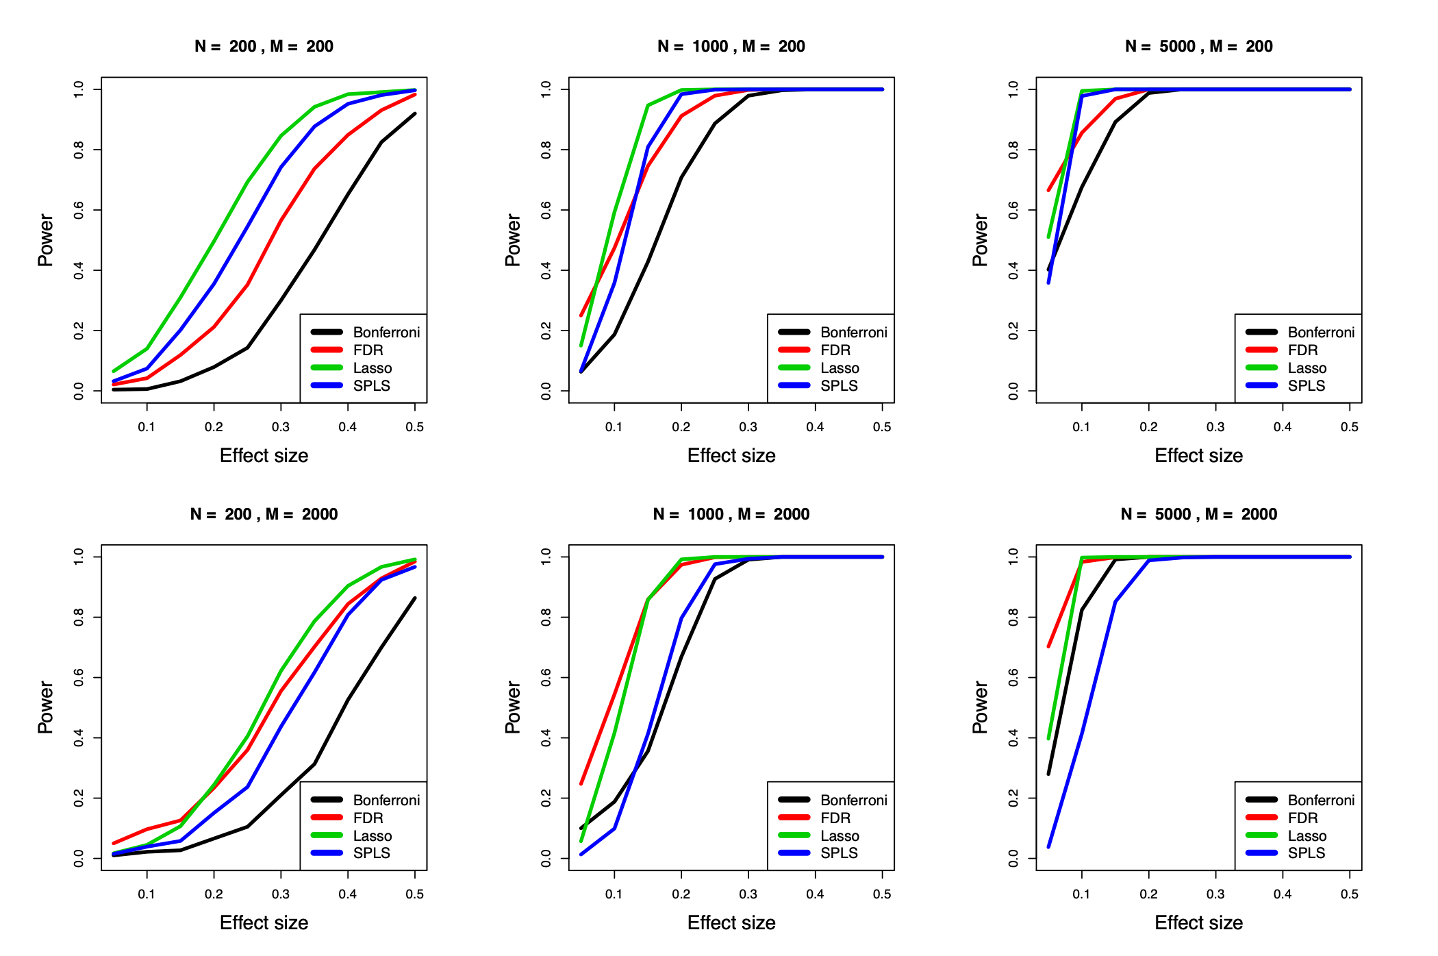
\includegraphics[keepaspectratio]{images/univariate_simulation.png}}

}

\caption{Henglin, M. et al.~(2022), ``Quantitative Comparison of
Statistical Methods for Analyzing Human Metabolomics Data,''
Metabolites, 12, 519.}

\end{figure}%

\note{Peluso et al.~2021: ``\ldots the complex non-normal structure of
metabolic profiles and outcomes may bias the permutation results leading
to overly conservative threshold estimates\ldots{}''

``Henglin et al.~2022 ``We observed that when the number of metabolites
was similar to or exceeded the number of study subjects, as is common
with nontargeted metabolomics performed in small cohorts, sparse
multivariate models demonstrated the most consistent results and the
most statistical power.''\,''}
\end{frame}

\begin{frame}{Prior work}
\phantomsection\label{prior-work}
\begin{figure}[H]

{\centering \includegraphics[width=0.8\linewidth,height=\textheight,keepaspectratio]{jsm-2025_files/mediabag/x1.png}

}

\caption{Zhang, E. et al.~(2025),
\href{https://doi.org/10.48550/arXiv.2502.10648}{``LLM-Lasso: A Robust
Framework for Domain-Informed Feature Selection and Regularization,''}
arXiv.}

\end{figure}%

\begin{figure}[H]

{\centering \pandocbounded{\includegraphics[keepaspectratio]{jsm-2025_files/mediabag/x11.png}}

}

\caption{Capstick, A. et al.~(2025),
\href{https://doi.org/10.48550/arXiv.2411.17284.}{``AutoElicit: Using
Large Language Models for Expert Prior Elicitation in Predictive
Modelling,''} arXiv.}

\end{figure}%
\end{frame}

\section{Methods}\label{methods}

\begin{frame}{Prior elicitation framework overview}
\phantomsection\label{prior-elicitation-framework-overview}
\pandocbounded{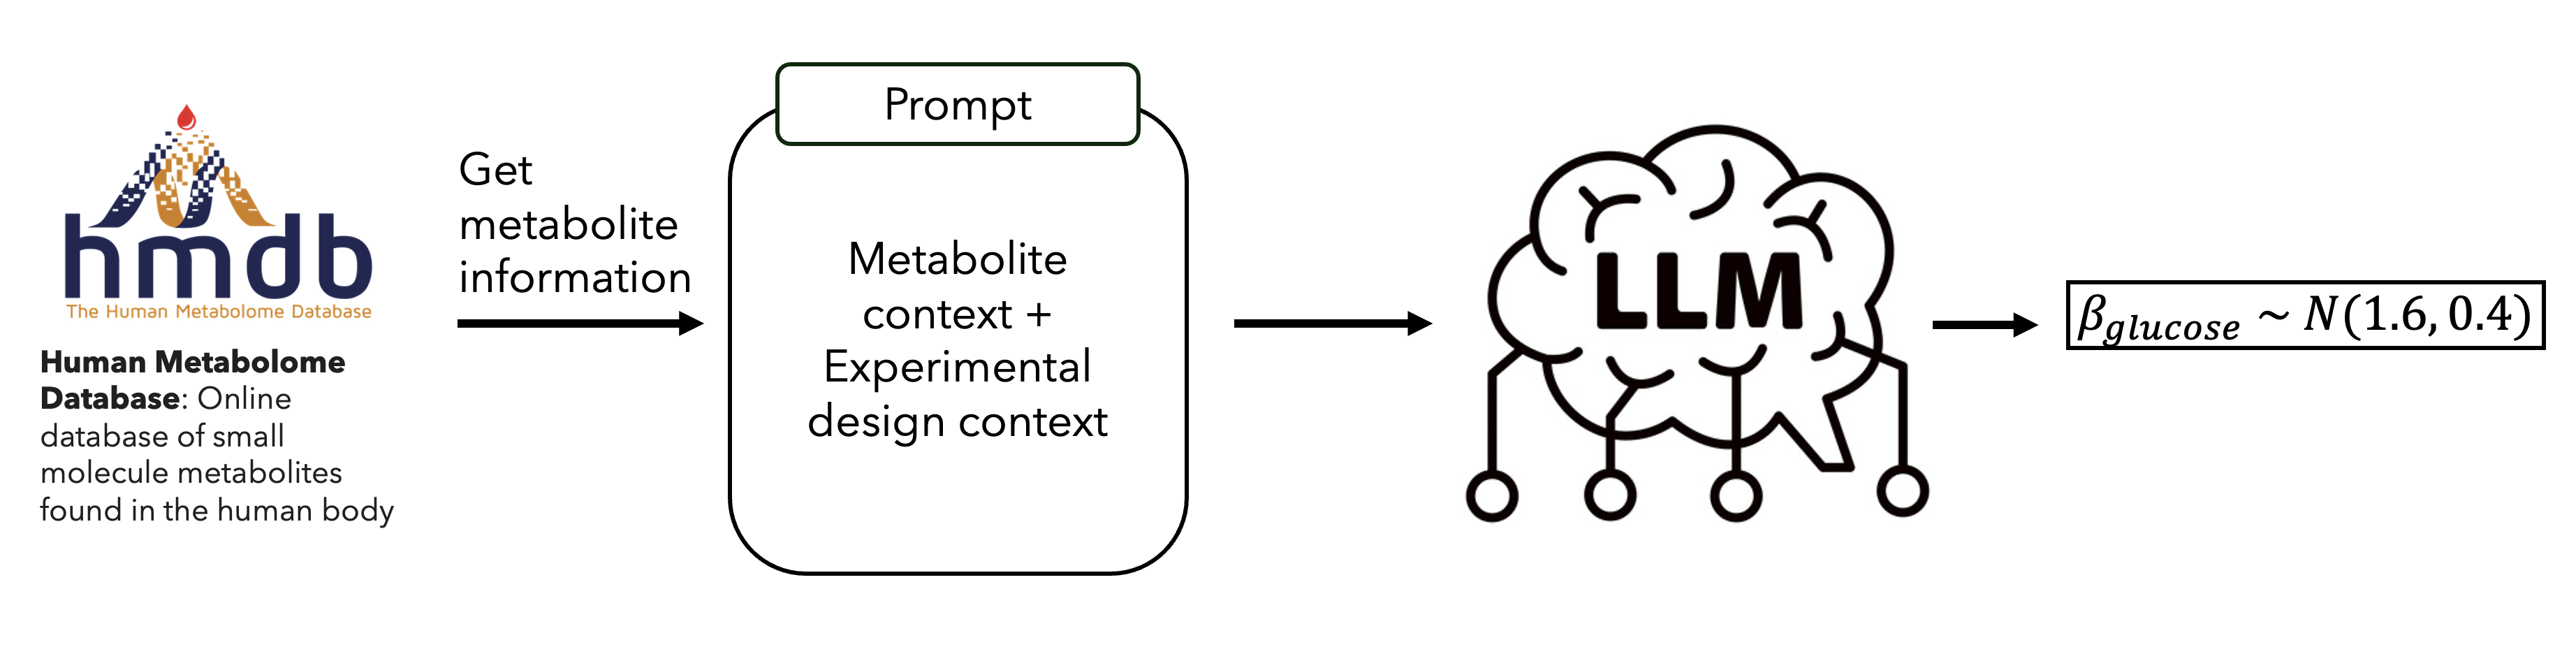
\includegraphics[keepaspectratio]{./images/overview.png}}

\begin{itemize}
\tightlist
\item
  \textbf{Metabolite Context Enrichment}: HMDB database integration for
  biological context (pathways, functions, disease associations)
\item
  \textbf{Multi-Model LLM Support}: OpenAI (GPT-4o, O3), Google (Gemini
  2.0/2.5), with caching and fallback mechanisms
\item
  \textbf{Qualitative-to-Numerical Mapping}: Conservative/moderate
  strength mappings with magnitude-driven effect sizes and
  confidence-calibrated uncertainties
\item
  \textbf{Hierarchical Bayesian Modeling}: LLM-informed metabolite
  grouping with intelligent pooling and minimal shrinkage
\item
  \textbf{Benchmark Framework}: Monte Carlo subsampling against ground
  truth with bias-variance decomposition
\end{itemize}
\end{frame}

\begin{frame}{LLM prior elicitation process}
\phantomsection\label{llm-prior-elicitation-process}
\textbf{Step 1}: LLM analyzes metabolite + study context
\[\text{LLM}(\text{metabolite}, \text{condition}) \rightarrow \{d_j, m_j, c_j, r_j\}\]

where \(d_j \in \{\text{increase, decrease, unchanged}\}\) is predicted
direction, \(m_j \in \{\text{small, moderate, large}\}\) is predicted
magnitude, \(c_j \in \left(0, 1\right)\) is confidence level, and
\(r_j\) is a string representing the rationale.

\textbf{Step 2}: Map qualitative predictions to numerical priors

\begin{align*}
\mu_j^{\text{LLM}} &= f_{\mu}\left(m_j, d_j\right) \\
\sigma_j^{\text{LLM}} &= f_{\sigma}\left(c_j\right)
\end{align*}

\textbf{Step 3}: Use as informative priors in Bayesian model
\(\beta_j \sim \mathcal{N}(\mu_j^{\text{LLM}}, \sigma_j^{\text{LLM}})\)
\end{frame}

\begin{frame}{Priors}
\phantomsection\label{priors}
\textbf{LLM Priors}:
\(\beta_j \sim \mathcal{N}(\mu_j^{\text{LLM}}, \sigma_j^{\text{LLM}})\)

where \(\mu_j^{\text{LLM}}\) and \(\sigma_j^{\text{LLM}}\) are derived
from LLM predictions:

\begin{align}
\mu_j^{\text{LLM}} &= m_j \cdot \text{sign}(d_j) \\
\sigma_j^{\text{LLM}} &= f(c_j)
\end{align}

\textbf{Conservative Mapping}

\(m_j \in \{0.08, 0.15, 0.25\}\) for
\(\{\text{small, moderate, large}\}\)

\(f(c_j) \in \{0.5, 0.7, 0.9\}\) for \(\{\text{high, med, low}\}\)
confidence

\textbf{Moderate Mapping} \(m_j \in \{0.12, 0.22, 0.35\}\) for
\(\{\text{small, moderate, large}\}\)

\(f(c_j) \in \{0.3, 0.5, 0.7\}\) for \(\{\text{high, med, low}\}\)
confidence

\textbf{Oracle Prior (Upper Bound)}:
\(\beta_j \sim \mathcal{N}(\beta_j^{\text{true}}, 0.25)\)

\textbf{Weakly Informative Prior}: \(\beta_j \sim \mathcal{N}(0, 2)\)
\end{frame}

\begin{frame}{LLM-Informed Hierarchical Prior}
\phantomsection\label{llm-informed-hierarchical-prior}
Group metabolites by LLM predictions and use intelligent pooling:

\begin{align*}
\text{Group means}_g &\sim \mathcal{N}\bigl(\mu_g^{\mathrm{LLM}}, 3.0\bigr) \\
\beta_j &\sim \mathcal{N}\bigl(\text{Group means}_{g[j]}, 2.0\bigr)
\end{align*}

where group \(g\) is mapped to \(\mu_g^{\mathrm{LLM}}\) as follows:

\begin{align*}
\mu_g^{\mathrm{LLM}} =
\begin{cases}
-0.1, & \text{if }g = \text{decrease},\\
0.0,  & \text{if }g = \text{unchanged},\\
+0.1, & \text{if }g = \text{increase}.
\end{cases}
\end{align*}
\end{frame}

\begin{frame}{Modeling}
\phantomsection\label{modeling}
All Bayesian models use the same log-link GLM structure with different
prior specifications:

\begin{align}
y_{ij} &\sim \mathcal{N}(\mu_{ij}, \sigma_j^2) \\
\log(\mu_{ij}) &= \alpha_j + \beta_j \cdot x_i \\
\alpha_j &\sim \mathcal{N}(\log(\bar{y}_j + \epsilon), 1.0) \\
\sigma_j &\sim \text{HalfNormal}(0.5)
\end{align}

where \(y_{ij}\) is abundance for sample \(i\) and metabolite \(j\),
\(x_i \in \{0,1\}\) is group indicator, \(\beta_j\) represents the
natural log fold change (lnFC) for metabolite \(j\), and \(\epsilon\) is
a small constant to avoid log(0).
\end{frame}

\begin{frame}{Simulation Study}
\phantomsection\label{simulation-study}
\begin{block}{Empirical Monte-Carlo Subsampling}
\phantomsection\label{empirical-monte-carlo-subsampling}
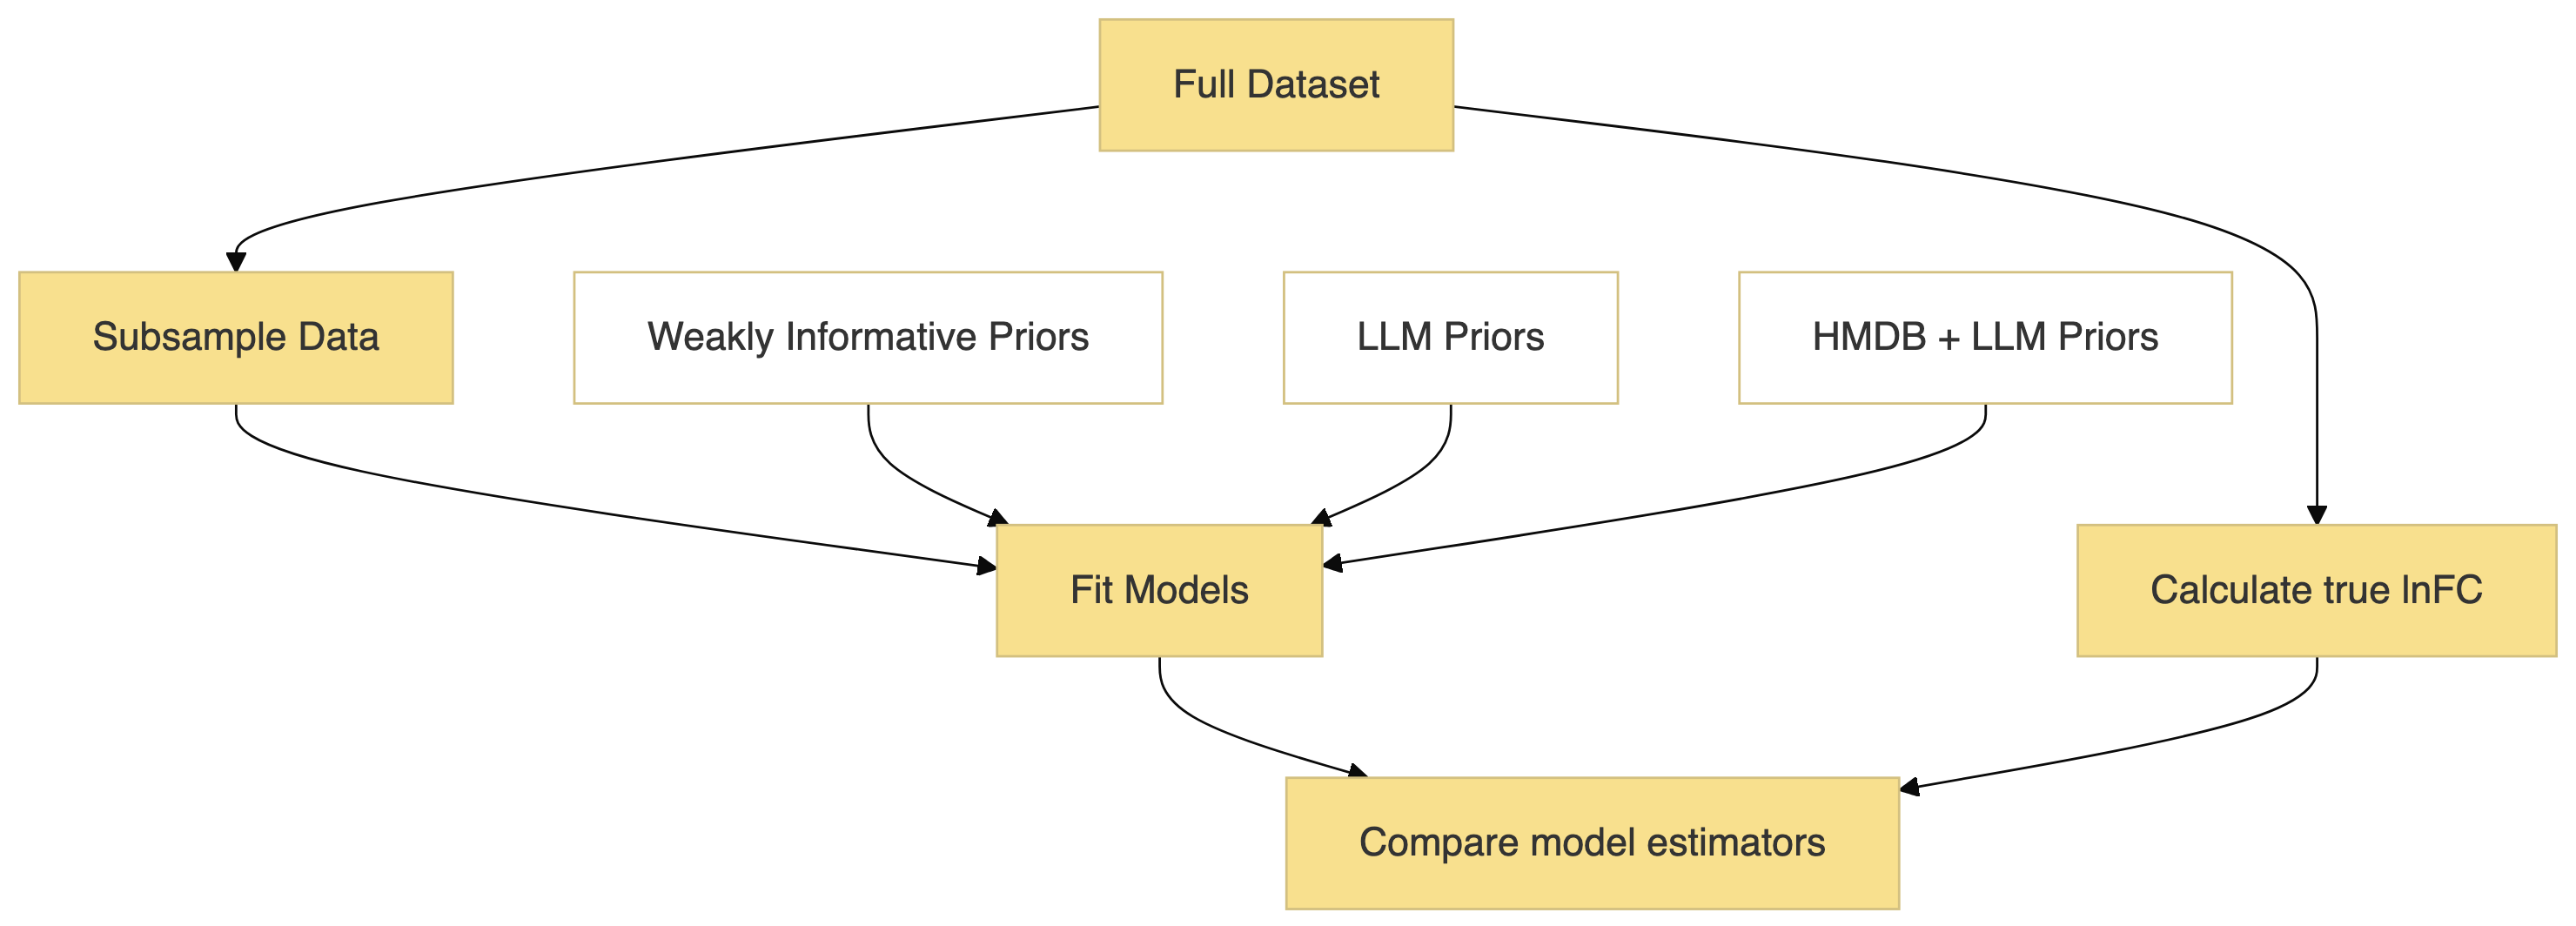
\includegraphics[width=8.32in,height=3in]{jsm-2025_files/figure-beamer/mermaid-figure-1.png}

\textbf{Ground Truth}: Empirical natural log fold change (lnFC) from
full MTBLS1 dataset\footnote<.->[frame]{Salek, R. M., Maguire, M. L.,
  Bentley, E., Rubtsov, D. V., Hough, T., Cheeseman, M., Nunez, D.,
  Sweatman, B. C., Haselden, J. N., Cox, R. D., Connor, S. C., and
  Griffin, J. L. (2007),
  \href{https://doi.org/10.1152/physiolgenomics.00194.2006.}{``A
  metabolomic comparison of urinary changes in type 2 diabetes in mouse,
  rat, and human,''} Physiological Genomics, American Physiological
  Society.} (n=132)

\[\beta_j^{\text{true}} = \log\left(\frac{\bar{y}_j^{\text{case}}}{\bar{y}_j^{\text{control}}}\right)\]
\end{block}
\end{frame}

\section{Results}\label{results}

\begin{frame}{LLM-informed priors improve recovery}
\phantomsection\label{llm-informed-priors-improve-recovery}
\pandocbounded{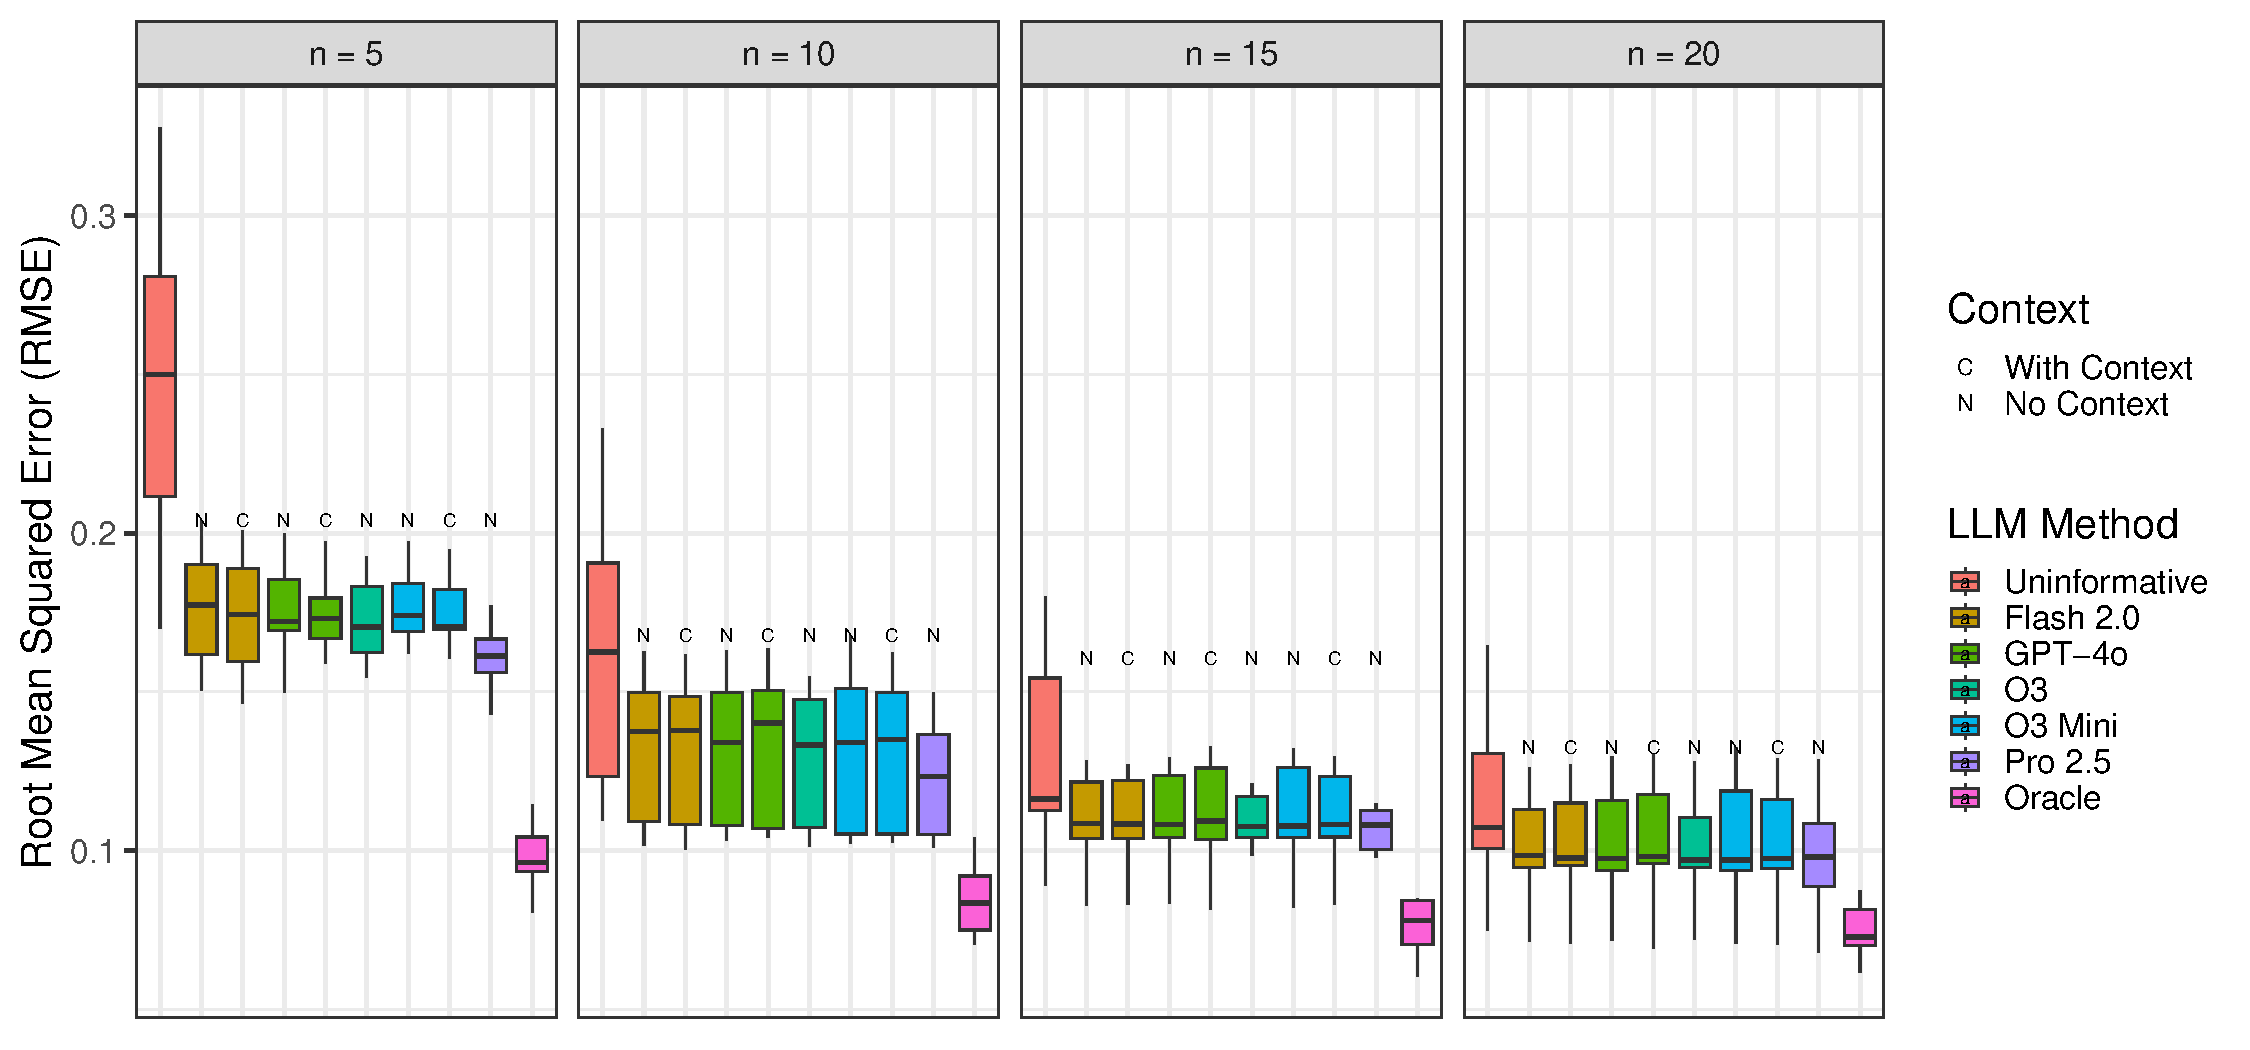
\includegraphics[keepaspectratio]{jsm-2025_files/figure-beamer/unnamed-chunk-2-1.pdf}}

\[\text{RMSE} = \sqrt{\frac{1}{n} \sum_{j=1}^{n} (\hat{\beta}_j - \beta_j^{\text{true}})^2}\]

where \(\hat{\beta}_j\) is the estimated effect size and
\(\beta_j^{\text{true}}\) is the ground truth lnFC for metabolite
\(m_j\).
\end{frame}

\begin{frame}{LLM Informed estimators are finite-sample efficient}
\phantomsection\label{llm-informed-estimators-are-finite-sample-efficient}
\pandocbounded{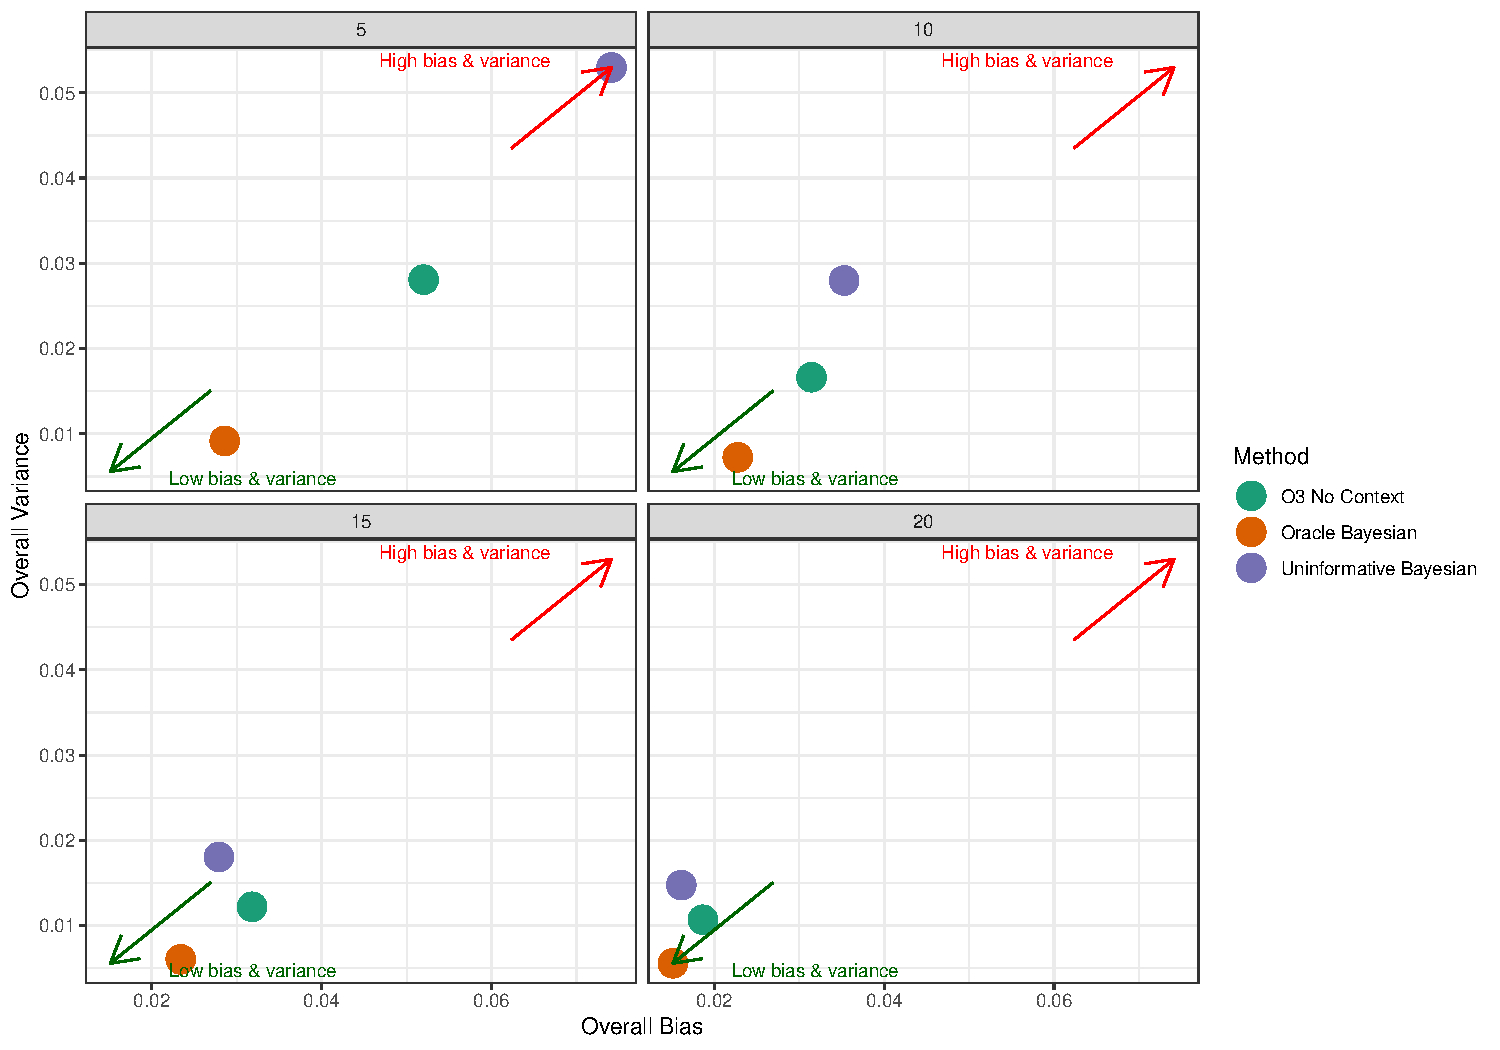
\includegraphics[keepaspectratio]{jsm-2025_files/figure-beamer/unnamed-chunk-3-1.pdf}}
\end{frame}

\begin{frame}{Summary}
\phantomsection\label{summary}
\begin{itemize}
\tightlist
\item
  \textbf{LLM Prior Elicitation Works}: Automated biological knowledge
  extraction via LLMs produces informative priors for Bayesian
  metabolomics analysis.
\item
  \textbf{Mapping Strategy Matters}: Magnitude-driven effect sizes and
  confidence-calibrated uncertainties are crucial for translating
  qualitative LLM insights into effective numerical priors.
\item
  \textbf{Added Context May Not Matter}: Including biological context
  from the HMDB in LLM prompts did not significantly improve prior
  performance in this study.
\item
  \textbf{Performance is Model Agnostic}: Different LLMs (OpenAI,
  Google) yielded similar results, indicating robustness across models.
\item
  \textbf{Practical Impact}: Method particularly valuable for small
  sample studies (n=5-20) where traditional statistical approaches
  struggle with high-dimensional metabolomics data.
\item
  \textbf{Future Directions}: Integration of other databases, alongside
  more sophisticated mapping approaches and historical data.
\end{itemize}
\end{frame}




\end{document}
